%! Author = Len Washington III
%! Date = 9/04/24

% Preamble
\documentclass[
	number={3},
	title={Na\"iive Bayes Learning}
]{cs584notes}

% Document
\begin{document}

\section{Direct Learning}\label{sec:direct-learning}
\begin{itemize}
	\item Consider a \emph{distribution} \data{$D$}
	\item \data{$X$} - \emph{Instance} space, \data{$Y$} - Set of \emph{labels}. (e.g. \data{$\pm1$})
	\item Given a \emph{sample} \data{$\{ (\vec{x},y) \}_{1}^{n}$} and a \emph{loss function} \data{$L(\vec{x},y)$}, find a \emph{hypothesis} \data{$h \in H$} that minimizes \data{$\sum_{i=1\dots n} L(h(\vec{x}_{i}), y_{i})$}.
\end{itemize}

\begin{table}[H]
	\centering
	\caption{Losses}
	\label{tab:losses}
	\begin{tabular}{l l}
		0 -- 1 loss: & \data{$L(h(\vec{x}), y) = 1, h(\vec{x}) \neq y$ otherwise $L(h(\vec{x}), y) = 0$}\\
		$L_{2}$ Loss: & \data{$L(h(\vec{x}), y) = \left( h(\vec{x}) - y \right)^{2}$}\\
		Hinge Loss: & \data{$L(h(\vec{x}), y) = \max\{ 0, 1 - yh(\vec{x}) \}$}\\
		Exponential Loss: & \data{$L(h(\vec{x}), y) = e^{-yh(\vec{x})} $}\\
	\end{tabular}
\end{table}

\section{Probabilistic Model}\label{sec:probabilistic-model}
Paradigm:
\begin{itemize}
	\item \emph{Learn} a \emph{probability distribution} of the \emph{dataset}.
	\item Use it to \emph{estimate} which outcome is more likely.
\end{itemize}

Instead of learning \data{$h: X\rightarrow Y$}, \emph{learn} \data{$P(Y|X)$}.

\begin{itemize}
	\item Estimate probability from data
	\begin{itemize}
		\item Maximum Likelihood Estimate (MLE)
		\item Maximum Aposteriori Estimation (MAP)
	\end{itemize}
\end{itemize}

\section{Probability Recap}\label{sec:probability-recap}
\begin{gather*}
    0 \leq P(A) \leq 1\\
    P(true) = 1, P(false) = 0\\
    P(A \lor B) = P(A) + P(B) + P(A \land B)\\
    P(A|B) = \frac{P(A\land B)}{{P(B)}}\\
\end{gather*}

\section{Joint Distribution}\label{sec:joint-distribution}
Making a \emph{joint distribution} of \data{$d$} \emph{variables}
\begin{itemize}
	\item Make a \emph{truth table} listing all combinations of values of your variables (if there are \data{$d$} \emph{boolean variables} then the table will have \data{$2^{d}$ rows})
	\item For \emph{each combination} of values, say how \emph{probable} it is.
	\item The \emph{probability} must \emph{sum} up to \data{$1$}.
\end{itemize}

Once we have the Joint Distribution, we find probability of any logical expression involving these variables.

\[ \data{P(E) = \sum_{rows\ matching\ E}P(row)} \]

\begin{equation}
	\begin{aligned}
		P(E_{1}\ |\ E_{2}) &= \frac{E_{1} \land E_{2}}{P(E_{2})}\\
		&= \frac{\sum_{\mbox{rows matching } E_{1} \mbox{ and } E_{2}}P(row)}{\sum_{\mbox{rows matching } E_{2}}P(row)}
	\end{aligned}
	\label{eq:evidence-based-probability}
\end{equation}

\section{Probability Distribution}\label{sec:probability-distribution}
\subsection{Bernoulli Distribution}\label{subsec:bernoulli-distribution}
Random Variable \data{$X$} takes values \data{$\{0, 1\}$} such that
\[ \data{ P(X=1) = p = 1 - P(X=0) } \]
Example: Tossing a coin.

\subsection{Binomial Distribution}\label{subsec:binomial-distribution}
Random Variable \data{$X$} takes values \data{$\{ 1, 2, \dots, n\}$} representing the number of successes \data{$X=1$} in \data{$n$} Bernoulli trials.
\[ \data{ P(X = k) = f(n, p, k) = C_{n}^{k}p^{k}(1 - p)^{n-k} } \]
Example: Tossing a coin \data{$n$} times.

\subsection{Categorical Distribution}\label{subsec:categorical-distribution}
Random Variable \data{$X$} takes on values in \data{$\{ 1, 2, \dots, k \}$} such that
\[ \data{ P(X = i) = p_{i} } \mbox{ and } \data{ \sum_{1}^{k} p_{i} = 1 } \]
Example: Rolling a die.

\subsection{Multinomial Distribution}\label{subsec:multinomial-distribution}
\begin{itemize}
	\item Let the random variables \data{$X_{i}(i = 1, 2, \dots, k)$} indicates the number of times outcome \data{$i$} was observed over the \data{$n$} trials.
	\item The vector $X=(X_{1}, X_{2}, \dots, X_{k})$ follows a multinomial distribution \data{$(n, p)$} where \data{$p = (p_{1}, p_{2}, \dots, p_{k})$} and \data{$\sum_{1}^{k} = 1$}
	\data{\begin{equation*}
	\begin{aligned}
		f(x_{1}, x_{2}, \dots, x_{k}, n, p) &= P(X_{1} = x_{1}, X_{2} = x_{2}, \dots, X_{k} = x_{k})\\
											&= \frac{n!}{x_{1}! \times x_{2}! \times \dots \times x_{k}!} \times p_{1}^{x_{1}} \times p_{2}^{x_{2}} \times \dots \times p_{k}^{x_{k}} \mbox{ where } \sum_{i=1}^{k} x_{i} = n
	\end{aligned}
	\end{equation*}}
\end{itemize}
Example: Rolling a die \data{$n$} times.

\section{Independence}\label{sec:independence}
When two \emph{events} do \emph{not affect} each other's \emph{probabilities}, they are called \emph{independent events}

\data{\begin{equation*}
\begin{aligned}
	A \upvDash B &\leftrightarrow P(A\land B) = P(A)\times P(B)\\
				 &\leftrightarrow P(A\ |\ B) = P(A)\\
\end{aligned}
\end{equation*}}

The \emph{conditional independence} of events \data{$A$} and \data{$B$}, given \data{$C$} is:
\data{\begin{equation*}
\begin{aligned}
	A \upvDash B | C \leftrightarrow P(A\ |\ B,C) &= \frac{P(A\land B|C)}{P(B|C)} = \frac{P(A|C)\times P(B|C)}{P(B|C)}\\
		&= P(A|C)
\end{aligned}
\end{equation*}}

\section{Bayes' Rule}\label{sec:bayes'-rule}
\begin{equation}
	\data{P(A|B) = \frac{P(B|A)\times P(A)}{P(B)}}
	\label{eq:bayes-rule}
\end{equation}
where \data{$A$} and \data{$B$} are \emph{events} and \data{$P(B)\neq0$}.
Applying \emph{Bayes' rule} for \emph{machine learning} --

\begin{equation}
	\data{P(hypothesis\ |\ evidence) = \frac{P(evidence\ |\ hypothesis)\times P(hypothesis)}{P(evidence)}}
	\label{eq:bayes-rule-ml}
\end{equation}

\section{Bayesian Learning}\label{sec:bayesian-learning}
\begin{itemize}
	\item Goal: find the \emph{best hypothesis} from some space \data{$H$} of \emph{hypotheses}, given the observed data (\emph{evidence}) \data{$D$}.
	\item Define the \emph{most probable hypothesis} in \data{$H$} to be the \emph{best}.
	\item In order to do that, we need to \emph{assume} a \emph{probability distribution} over the \emph{class} \data{$H$}.
	\item In addition, we need to know something about the \emph{relation} between the \emph{evidence} and the \emph{hypotheses}.
\end{itemize}

\begin{description}[font=\color{red}]
	\item[$P(h)$] -- \emph{Prior Probability} of the \emph{hypothesis} \data{$h$}. Reflects the background knowledge, before data is observed.
	\item[$P(D)$] -- \emph{Probability} that this sample of the \emph{data} is \emph{observed}.
	\item[$P(D|h)$] -- {Probability} of \emph{observing} the \emph{sample} \data{$D$}, given that \emph{hypothesis} $h$ is the \emph{target}, also referred to as \emph{likelihood}.
	\item[$P(h|D)$] -- \emph{Posterior probability} of \data{$h$}. The \emph{probability} that \data{$h$} is the \emph{target}, given that \data{$D$} has been \emph{observed}.
\end{description}

\begin{itemize}
	\item \data{$P(h|D)$} \emph{increases} with \data{$P(h)$} and \data{$P(D|h)$}.
	\item \data{$P(h|D)$} \emph{decreases} with \data{$P(D)$}.
\end{itemize}

\section{Maximum APosteriori Estimate}\label{sec:maximum-aposteriori-estimate}
\data{\begin{equation}
	P(h|D) = \frac{P(D|h)\times P(h)}{P(D)}
	\label{eq:map}
\end{equation}}
\begin{itemize}
	\item The \emph{learner} considers a \emph{set of candidate hypotheses} \data{$H$} (models) and attempts to find the \emph{most probable} one \data{$h\in H$}, given the observed data.
	\item Such maximally probable hypothesis is called \emph{maximum a posterior estimate} (MAP). Bayes theorem is used to compute it:
	\data{\begin{equation*}
	\begin{aligned}
		h_{MAP} &= \arg\max_{h\in H}P(h|D)\\
				&= \arg\max_{h\in H}\frac{P(D|h)\times P(h)}{P(D)}\\
				&= \arg\max_{h\in H}P(D|h)\times P(h)\\%}
	\end{aligned}
	\end{equation*}}
\end{itemize}

\section{Maximum Likelihood Estimate}\label{sec:maximum-likelihood-estimate}
\begin{itemize}
	\item We may assume that \emph{a priori}, \emph{hypotheses} are \emph{equally probable.}
	\[ \data{ P(h_{i}) = P(h_{j}) \forall h_{i}, h_{j} \in H } \]
	\item With that assumption, we can treat \data{$\frac{P(h)}{P(D)}$} as a constant. We get the \emph{maximum likelihood estimate} (MLE):
	\begin{equation}[eqred]
		\begin{aligned}
			h_{MLE} &= \arg\max_{h\in H} \frac{P(D|h)\times P(h)}{P(D)}\\
					&= \arg\max_{h\in H} P(D|h)P(h)
		\end{aligned}
		\label{eq:mle}
	\end{equation}
	\item Here we just \emph{look for} the \emph{hypothesis} that \emph{best explains} the \emph{data}.
\end{itemize}

\section{Bayesian Classifier}\label{sec:bayesian-classifier}
\begin{itemize}
	\item \data{$f: \vec{X}\rightarrow Y$} where, instances \data{$\vec{x}\in \vec{X}$} is a collection of inputs --
	\[ \data{ \vec{x} = (x_{1}, x_{2}, \dots, x_{n}) } \]
	\item Given an example, \emph{assign} it the \emph{most probable} value in \data{$Y$}.
	\begin{equation}[eqpurple]
	\begin{aligned}
		y_{MAP} &= \arg\max_{y_{j}\in Y} P(y_{j} | x)\\
				&= \arg\max_{y_{j}\in Y} P(y_{j} | x_{1}, x_{2}, \dots, x_{n})\\
				&= \arg\max_{y_{j}\in Y} \frac{P(x_{1}, x_{2}, \dots, x_{n}|y_{j})P(y_{j})}{P(x_{1}, x_{2}, \dots, x_{n})}\\
				&= \arg\max_{y_{j}\in Y} P(x_{1}, x_{2}, \dots, x_{n}|y_{j})P(y_{j})
	\end{aligned}
	\end{equation}
	\item Given the training data, we have to \emph{estimate} the two terms.
	\item Estimating \data{$P(y)$} is easy, e.g., under the \emph{binomial distribution assumption}, \emph{count} the number of \emph{times} \data{$y$} appears in the training data.
	\item However, it is \emph{not feasible} to estimate \data{$P(x_{1}, x_{2}, \dots, x_{n} | y)$}
	\item In this case, we have to \emph{estimate} for each \emph{target} value, the \emph{probability} of \emph{each instance} (some of which might now ever occur).
	\item In order to use a Bayesian classifiers in practice, we need to \emph{make assumptions} that will \emph{allow} us to \emph{estimate} these quantities.
\end{itemize}

\section{Na\:ive Bayes Classifier}\label{sec:naive-bayes-classifier}
\emph{Assumption}: Input feature values are independent, given the target value.
\begin{equation}[eqpurple]
\begin{aligned}
	P(x_{1}, x_{2}, \dots, x_{n} | y_{j}) &= P(x_{1} | y_{j}) \times P(x_{2}, \dots, x_{n}, x_{j})\\
										  &= P(x_{1} | y_{j}) \times P(x_{2} | y_{j}) \times P(x_{3}, \dots, x_{n}, x_{j})\\
										  &= P(x_{1} | y_{j}) \times P(x_{2} | y_{j}) \times P(x_{3} | y_{j}) \times \dots \times P(x_{n} | x_{j})\\
	&= \data{ \prod_{i=1}^{n} P(x_{i} | y_{j}) }
\end{aligned}
	\label{eq:naive-bayes-classifier-proof}
\end{equation}

\begin{equation}
	\begin{aligned}
	Y_{NB} &= \arg\max_{y_{j} \in Y} P(x_{1}, x_{2}, \dots, x_{n} | y_{j})P(y_{j})\\
		   &= \arg\max_{y_{j} \in Y} P(y_{j})\prod_{i=1}^{n} P(x_{i} | y_{j})\\
	\end{aligned}
	\label{eq:naive-bayes-classifier}
\end{equation}

\section{Estimating Probabilities}\label{sec:estimating-probabilities}
How do we estimate \data{$P(x_{i} | y)$}?
\begin{equation}
	P(x_{i} | y) = \frac{\mbox{number of } x_{i} \mbox{ labeled as } y}{\mbox{ total number of label } y} = \frac{n_{i}}{n}
	\label{eq:estimating-probabilities}
\end{equation}
\emph{Sparsity} of data is a problem --
\begin{itemize}
	\item If \data{$n$} is \emph{small}, the estimate is not accurate.
	\item If \data{$n_{i} = 0$}, we will never accurately predict \data{$Y$} if an \emph{instance} that \emph{never appeared} in the \emph{training} appears in the test data.
\end{itemize}

\section{Laplace Smoothing}\label{sec:laplace-smoothing}
\begin{equation}
	P(x_{i} | y) = \frac{n_{i} + \alpha}{n + \alpha d}
	\label{eq:laplace-smoothing}
\end{equation}
\begin{itemize}
	\item Also known as \emph{additive smoothing}.
	\item $\alpha > 0$ is a smoothing parameter.
	\item \data{$d$} is the \emph{dimension} of the input.
\end{itemize}

\section{Continuous Features}\label{sec:continuous-features}
\begin{itemize}
	\item Assume \data{$P(x_{i} | y)$} has a \emph{Gaussian (normal) distribution}.
	\item It is a continuous distribution with probability density function:
	\begin{equation}
		p(x) = \frac{1}{\sqrt{2\pi\sigma^{2}}}e^{-\frac{(x - \mu)^{2}}{2\sigma^{2}}}
		\label{eq:gaussian-distribution}
	\end{equation}
	\begin{itemize}
		\item \data{$\mu$} is the \emph{mean} of the distribution.
		\item \data{$\sigma^{2}$} is the \emph{variance} of the distribution.
		\item \data{$x$} is a \emph{continuous} variance \data{$(-\infty \leq x \leq \infty)$}
	\end{itemize}
\end{itemize}

\section{Gaussian Naïve Bayes}\label{sec:gaussian-naive-bayes}
\begin{table}[H]
	\centering
	\caption{\Naive Bayes Example}
	\label{tab:naive-bayes-Example}
	\rowcolors{2}{lightgreen}{medgreen}
	\begin{tabular}{c c c c}
		\rowcolor{darkgreen} \textcolor{white}{$X_{1}$} & \textcolor{white}{$X_{2}$} & \textcolor{white}{$X_{3}$} & \textcolor{white}{$Y$}\\
		2 & 3 & 1 & 1\\
		-1.2 & 2 & 0.4 & 1\\
		1.2 & 0.3 & 0 & 0\\
		2.2 & 1.1 & 0 & 1
	\end{tabular}
\end{table}


Compute the \emph{mean} and \emph{standard deviation} to estimate the \emph{likelihood}.

\begin{equation*}
	\begin{aligned}[eqpurple]
		\mu_{1} &= E[X_{1}\ |\ Y = 1] = \frac{2 + (-1.2)  + 2.2}{3} = 1\\
		\sigma_{1}^{2} &= E\left[ (X_{1} - \mu_{1})^{2} | Y = 1 \right] = \frac{(2-1)^{2} + (-1.2 - 1)^{2} + (2.2 - 1)^{2}}{3} = 2.43\\
		P(x_{1} | Y=1 ) &= \frac{1}{\sqrt{2\pi\sigma^{2}}}e^{-\frac{(x_{1} - \mu_{1})^{2}}{2\sigma^{2}}} = \frac{1}{3.91}e^{-\frac{(x_{1} - 1)^{2}}{4.86}}
	\end{aligned}
\end{equation*}

\section{Bayesian Belief Network}\label{sec:bayesian-belief-network}
\begin{itemize}
	\item Naïve Bayes classifier works with the \emph{assumption} that the values of the \emph{input features} are \emph{conditionally independent} given the \emph{target value}.
	\item This \emph{assumption} dramatically \emph{reduces} the \emph{complexity} of \emph{learning} the \emph{target function}.
	\item \emph{Bayesian Belief Network} describes the probability distribution governing a set of variables by specifying a \emph{set of conditional independence assumptions} along with a set of conditional probabilities. \emph{Conditional independence} assumptions here apply to \emph{subsets} of the \emph{variables}.
	\[ \data{ P(x_{1}, x_{2}, \dots, x_{l}\ |\ x_{1}{'}, x_{2}{`}, \dots, x_{m}{`}, y_{1}, y_{2}, \dots, y_{n}) = P(x_{1}, x_{2}, \dots, x_{l} | y_{1}, y_{2}, \dots, y_{n}) } \]
\end{itemize}

\section{Training Bayesian Classifier}\label{sec:training-bayesian-classifier}
During \emph{training}, typically \emph{log-space} is used.

\data{\begin{equation*}
		  \begin{aligned}
			  y_{NB} &= \arg\max_{y} \left[ \log P(y) \prod_{i=1}^{n} P(x_{i} | y) \right]\\
			  &= \arg\max_{y} \left[ \log P(y) + \sum_{i=1}^{n} \log P(x_{i} | y) \right]\\
		  \end{aligned}
\end{equation*}}

\section{Text Classification}\label{sec:text-classification}
\begin{algorithm}[H]
	\caption{Text-based Naïve Bayes Classification}\label{alg:train-naive-bayes}
	\begin{algorithmic}[1]
		\Function{Train-Naive-Bayes}{$D, C$} \Returns $\log P(c)$ and $\log P(w|c)$
			\ForAll{class $c\in C$}\Comment{Calculate $P(c)$ terms}
				\State $N_{doc} \gets$ number of documents in $D$
				\State $N_{c} \gets$ number of documents from $D$ in class $c$
				\State $logprior[c] \gets \log\frac{N_{c}}{N_{doc}}$
				\State $V \gets $ vocabulary of $D$
				\State $bigdoc[c] \gets \Call{Append}{d}$ \textbf{for} $d\in D$ \textbf{with} class $c$
				\ForAll{word $w$ in $V$}\Comment{Calculate $P(w|c)$ terms}
					\State $\Call{Count}{w,c}\gets $ \# of occurrences of $w$ in $bigdoc[c]$
					\State $loglikelihood[w, c]\gets \log \frac{\Call{Count}{w, c} + 1}{\sum_{w' \mbox{ in } V} (\Call{Count}{w', c} + |V|)} $
				\EndFor
			\EndFor
			\State \Return $logprior, loglikelihood, V$
		\EndFunction
	\end{algorithmic}
\end{algorithm}
\begin{algorithm}[H]
	\caption{Test \Naive Bayes}\label{alg:test-naive-bayes}
	\begin{algorithmic}[1]
	\Function{Test-Naive-Bayes}{$testdoc, logprior, loglikelihood, C, V$} \Returns best $c$
		\ForAll{class $c \in C$}
			\State $sum[c] \gets logprior[c]$
			\ForAll{position $i$ in $testdoc$}
				\State $word \gets testdoc[i]$
				\If{$word \in V$}
					\State $sum[c] \gets sum[c] + loglikelihood[word, c]$
				\EndIf
			\EndFor
		\EndFor
		\State \Return $\arg\max_{c}$, $sum[c]$
	\EndFunction
	\end{algorithmic}
\end{algorithm}

% TODO: Add practice
The word \emph{with} doesn't occur in the training set, so we drop it completely (we don't use unknown word models for Naïve Bayes)

\section{Evaluating Classifiers}\label{sec:evaluating-classifiers}
\begin{itemize}
	\item \emph{Gold Label} is the \emph{correct} output \emph{class} label of an input.
	\item \emph{Confusion Matrix} is a table for \emph{visualizing} how a \emph{classifier performs} with respect to the gold labels, using two dimensions (system output and gold labels), and each cell labeling a set of possible outcomes.
	\item \emph{True Positives} and \emph{True Negatives} are \emph{correctly classified} outputs belonging to the positive and negative class, respectively.
	\item \emph{False Positives} and \emph{False Negatives} are \emph{incorrectly classified} outputs.
\end{itemize}

\begin{figure}[H]
	\centering
	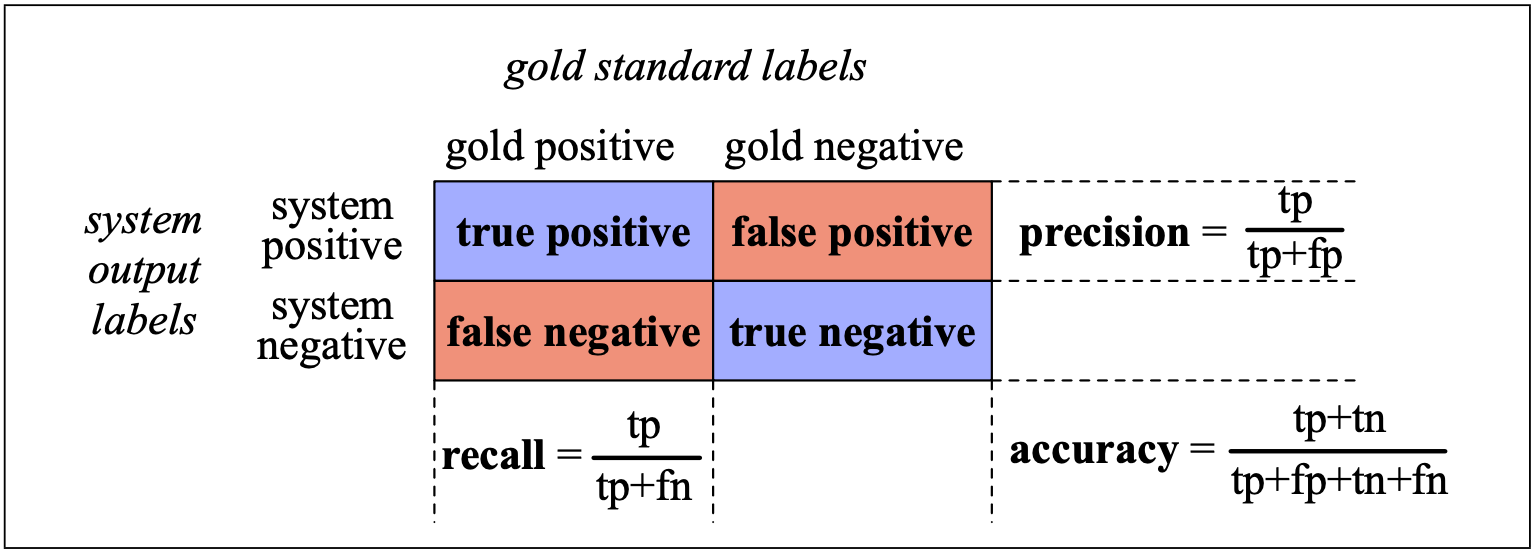
\includegraphics[width=\textwidth]{figures/3/confusion_matrix}
	\caption{An example of a Confusion Matrix.}
	\label{fig:confusion-matrix}
\end{figure}


\section{Precision, Recall, F-Measure}\label{sec:precision-recall-f-measure}
\begin{equation}
	\mathbf{Precision} = \frac{\mbox{true positives}}{\mbox{true positives } + \mbox{ false positives}}
	\label{eq:precision}
\end{equation}

\begin{equation}
	\mathbf{Recall} = \frac{\mbox{true positives}}{\mbox{true positives } + \mbox{ false negatives}}
	\label{eq:recall}
\end{equation}

\begin{equation}
	\mathbf{F-measure} = F_{\beta} = \frac{(\beta^{2} + 1)PR}{\beta^{2}P + R}\\
	\label{eq:f-measure}
\end{equation}

\section{ROC Curve}\label{sec:roc-curve}
\begin{itemize}
	\item A \emph{receiver operating characteristic} curve (ROC curve) is a graphical plot that illustrates the \emph{performance} of a \emph{binary classifier model}.
	\item The \emph{ROC curve} is the plot of the \emph{true positive rate (recall)} (TPR)~\eqref{eq:recall} against the \emph{false positive rate} (FPR).
	\begin{equation}
		\mathbf{FPR} = \frac{\mbox{false positives}}{\mbox{false positives } + \mbox{ true negatives}}
		\label{eq:fpr}
	\end{equation}
	\item \emph{ROC curve} plots \emph{TPR vs. FPR} at different \emph{classification thresholds}.
	\item \emph{Classification threshold} is used to convert the \emph{output} of a \emph{probabilistic classifier} into class \emph{labels}.
	\item The \emph{threshold} determines the \emph{minimum probability} required for a \emph{positive class}.
	\item Lowering the classification threshold classifiers more items as \emph{positive}, thus increasing both False Positives and True Positives.
\end{itemize}

\begin{minipage}[m]{0.475\textwidth}
	\begin{figure}[H]
		\centering
		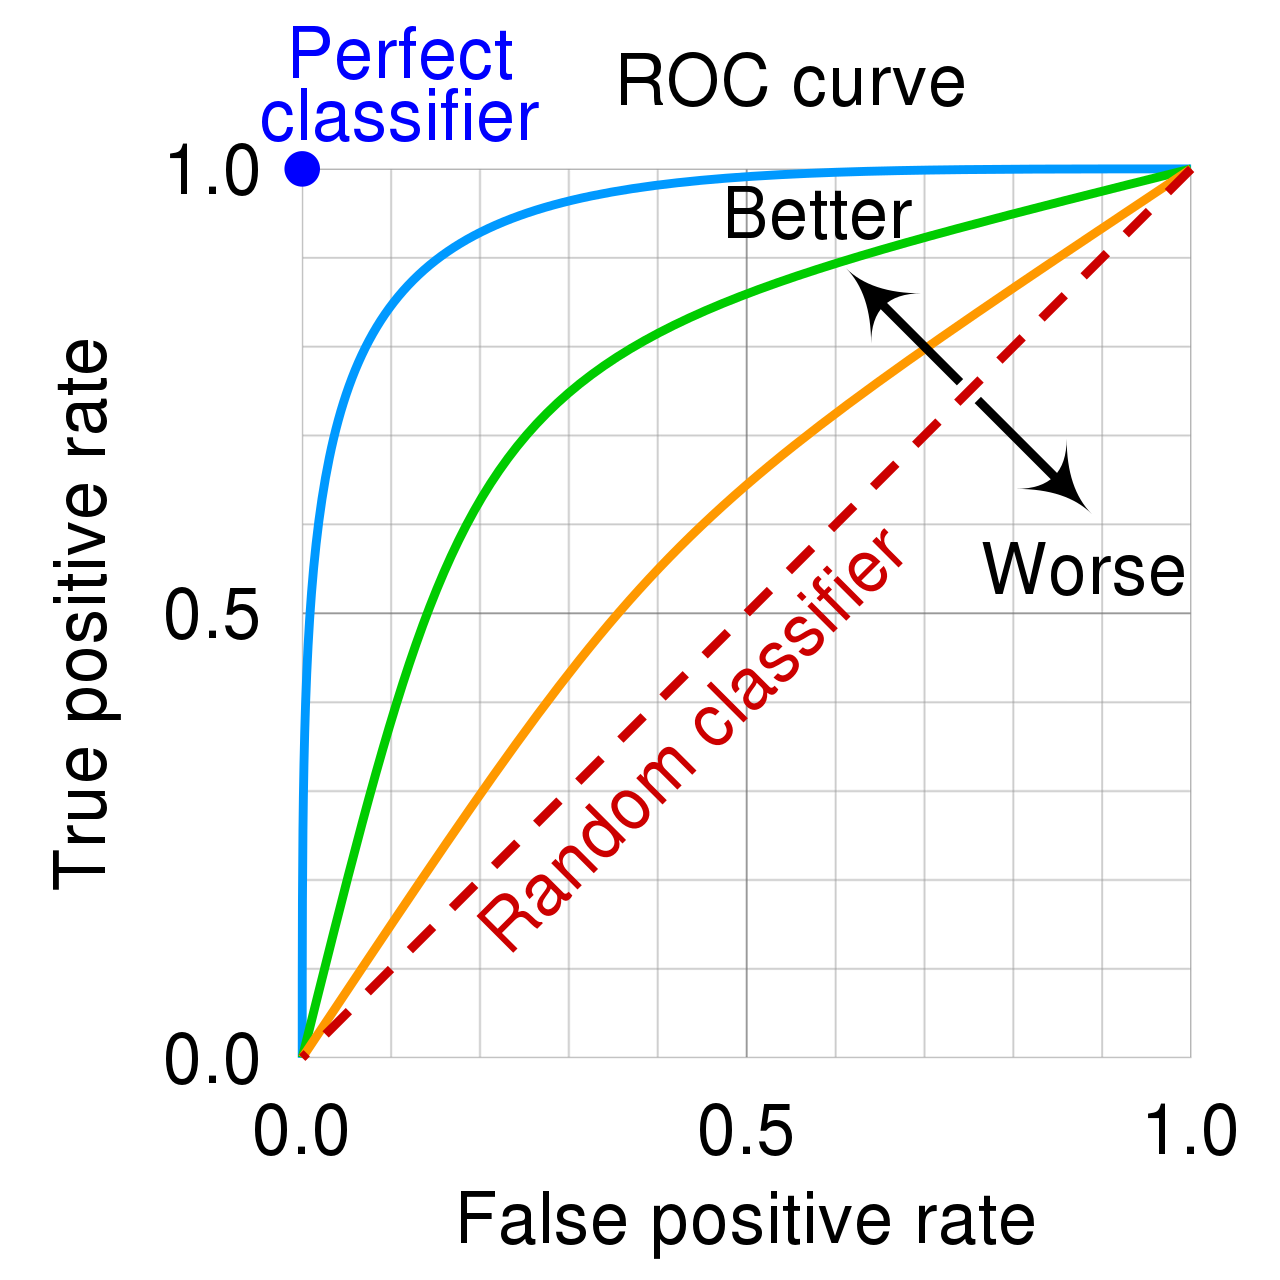
\includegraphics[width=\textwidth]{figures/3/roc_curve}
		\caption{ROC Curve}
		\label{fig:roc_curve}
	\end{figure}
\end{minipage}\hfill%
\begin{minipage}[m]{0.475\textwidth}
	\begin{figure}[H]
		\centering
		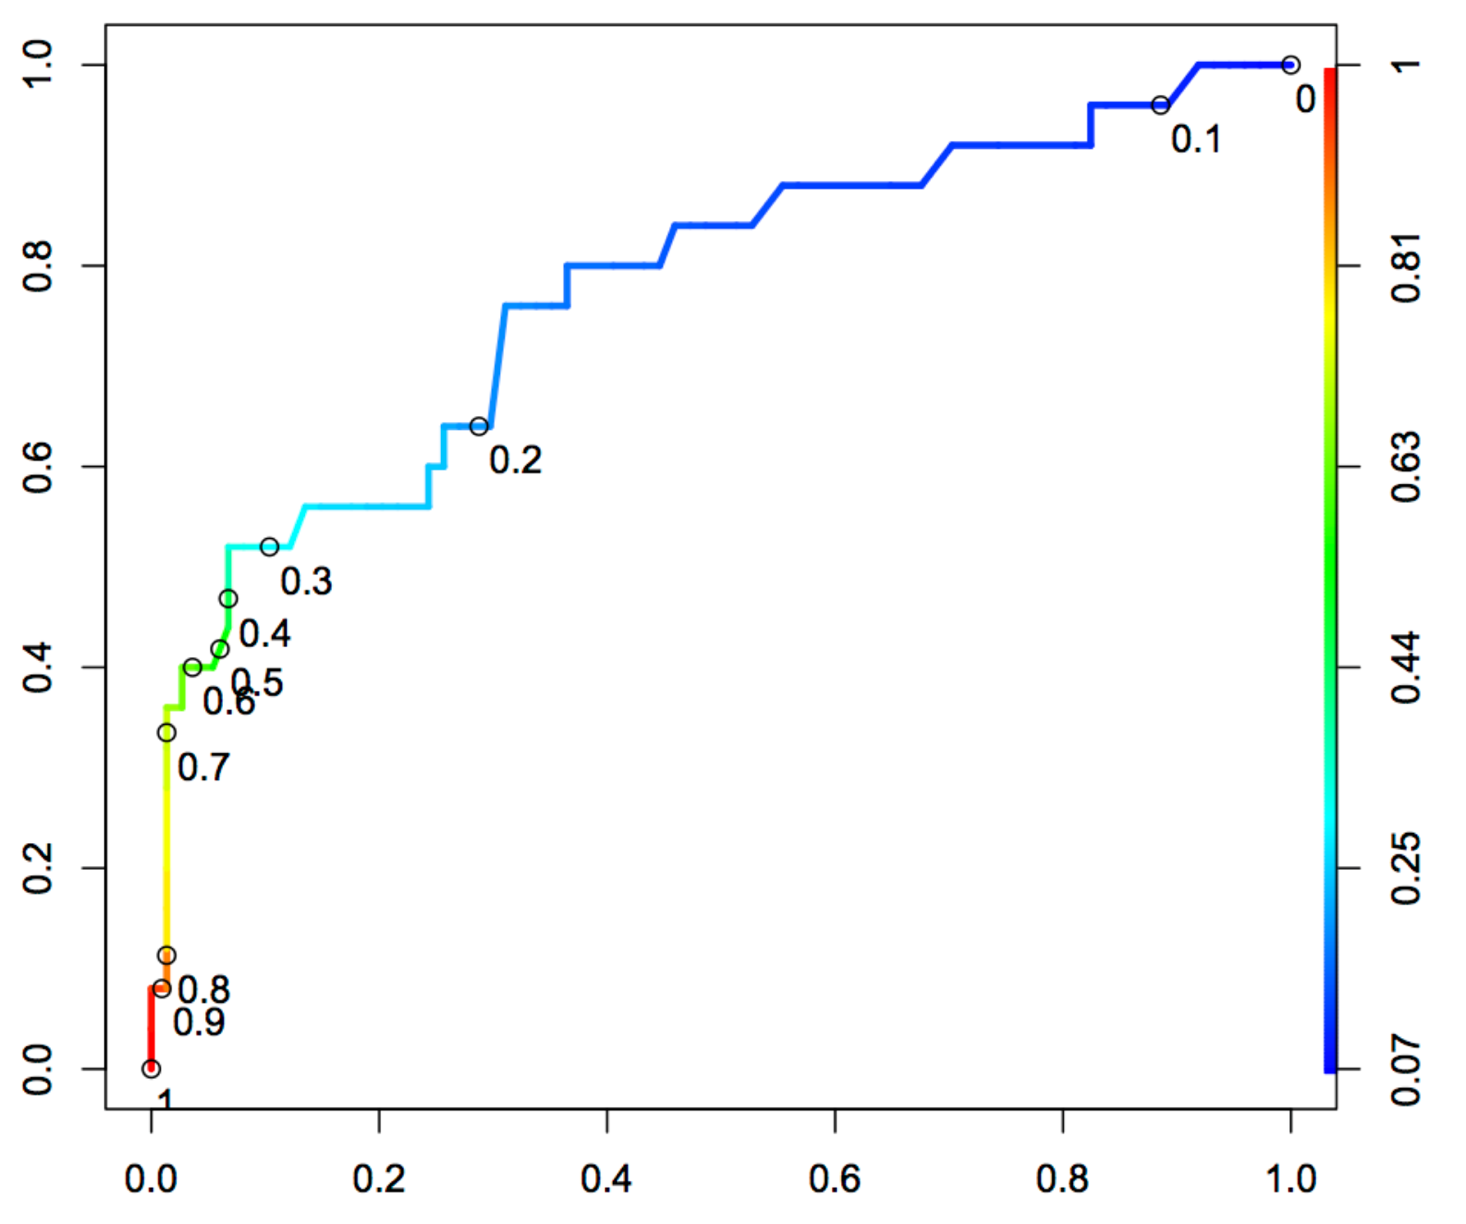
\includegraphics[width=\textwidth]{figures/3/rough_roc_curve}
		\caption{ROC Curve with defined thresholds}
		\label{fig:rough_roc_curve}
	\end{figure}
\end{minipage}

\section{AUC}\label{sec:auc}
\begin{itemize}
	\item The Area Under the Curve (AUC) provides an \emph{aggregate} measure of \emph{performance} across all possible classification thresholds.
	\item Between two ROC curves plotted based on two learning models, the model with the higher AUC \emph{learned better} than the other.
\end{itemize}

\section{\Naive Bayes: Two Classes}\label{sec:naive-bayes:-two-classes}
\begin{itemize}
	\item \Naive Bayes classifier gives a method for \emph{predicting} the \emph{most likely class} rather than an explicit class.
	\item In the case of two classes, \data{$y\in\{0, 1\}$} we predict that \data{$y=1$} iff
	\textcolor{eqpurple}{\begin{equation*}
		\frac{P(y_{j} = 1) \times \prod_{i=1}^{n} P(x_{i}|y_{j}=1)}{P(y_{j} = 0) \times \prod_{i=1}^{n} P(x_{i}|y_{j}=0)} > 1
	\end{equation*}}
	\item \data{$p_{i} = P(x_{i} | y_{j} = 1)$}, \data{$q_{i} = P(x_{i} | y_{j} = 0)$}. Assuming Bernoulli \Naive Bayes,
	\begin{equation*}
	\begin{aligned}[eqpurple]
		&\frac{P(y_{j} = 1) \times \prod_{i=1}^{n} p_{i}^{x_{i}} (1 - p_{i})^{1 - x_{i}}}{P(y_{j} = 0) \times \prod_{i=1}^{n} q_{i}^{x_{i}} (1 - q_{i})^{1 - x_{i}}} > 1\\
		\Rightarrow & \frac{P(y_{j} = 1) \times \prod_{i=1}^{n} (1 - p_{i})(p_{i} / 1 - p_{i})^{x_{i}}}{P(y_{j} = 0) \times \prod_{i=1}^{n} (1 - q_{i})(q_{i} / 1 - q_{i})^{x_{i}}} > 1\\
	\end{aligned}
	\end{equation*}
\end{itemize}

Take logarithm; we predict \data{$y=1$} iff

\begin{equation*}
\begin{aligned}[eqpurple]
	\log \frac{P(y_{j}=1)}{P(y_{j}=0)} + \sum_{i}\log \frac{1-p_{i}}{1-q_{i}} + \sum_{i}\left( \log\frac{p_{i}}{1-p_{i}} - \log\frac{q_{i}}{1-q_{i}} \right)x_{i} > 0
\end{aligned}
\end{equation*}

\begin{itemize}
	\item We get that \Naive Bayes is a \emph{linear separator} with --
	\begin{equation}[eqpurple]
		w_{i} = \log\frac{p_{i}}{1 - p_{i}} - \log\frac{q_{i}}{1 - q_{i}} = \log\frac{p_{i}(1-q_{i})}{q_{i}(1-p_{i})}
		\label{eq:naive-bayes-separator}
	\end{equation}
	\item NB classifier corresponds to a \emph{linear classifier} if the likelihood is from \emph{exponential family distributions} i.e., Bernoulli, binomial, Gaussian etc.
	\item In the case of two classes, we can say:
	\begin{equation*}
	\begin{aligned}[eqpurple]
		\log \frac{P(y_{j} = 1 | x)}{P(y_{j} = 0 | x)} = \sum_{i}\vec{w}_{i}\vec{x}_{i} + b
	\end{aligned}
	\end{equation*}
	\item but since \data{$P(y_{j} = 1|x) = 1 - P(y_{j} = 0 | x)$}, we get:
	\[ \textcolor{eqpurple}{ P(y_{j}=1|x) = \frac{1}{1+e^{-\left( \sum_{i}w_{i}x_{i} + b \right)}} } \]
	\item This is simply the \emph{logistic function}.
\end{itemize}

\end{document}
